% The center O=(0,0), the pole of the line at infinity, and the four antipodal pairs.
\documentclass[tikz,border=8pt]{standalone}
\usepackage{amsmath,amssymb}
\begin{document}
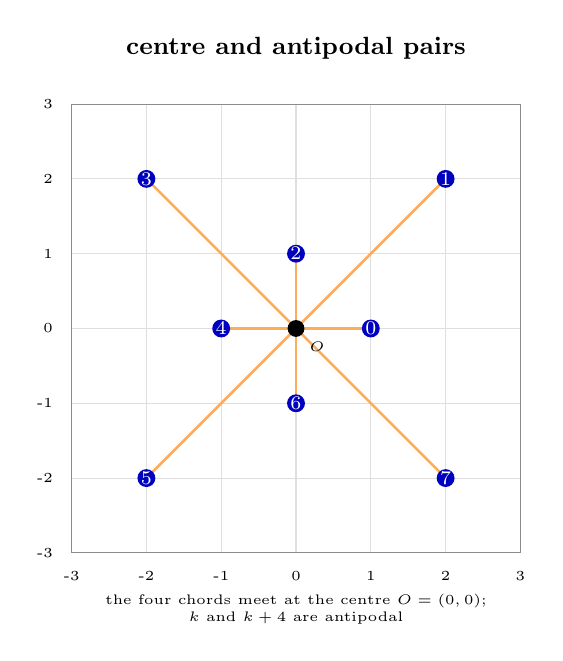
\begin{tikzpicture}[scale=0.95]
  \draw[gray!25] (-3,-3) grid (3,3);
  \draw[black!45] (-3,-3) rectangle (3,3);
  \foreach \x in {-3,...,3} {%
    \node[font=\tiny,below] at (\x,-3.12) {\x};%
    \node[font=\tiny,left] at (-3.12,\x) {\x};%
  }
  % four antipodal chords through the centre
  \foreach \x/\y in {1/0,2/2,0/1,-2/2} {%
    \draw[orange!65, line width=0.9pt] (\x,\y)--(-\x,-\y);}
  % centre
  \fill[black] (0,0) circle (3.2pt);
  \node[font=\tiny,below right] at (0.05,-0.05) {$O$};
  % the eight conic points
  \foreach \x/\y/\k in {1/0/0,2/2/1,0/1/2,-2/2/3,-1/0/4,-2/-2/5,0/-1/6,2/-2/7} {%
    \fill[blue!75!black] (\x,\y) circle (3.4pt);%
    \node[font=\scriptsize,text=white] at (\x,\y) {\k};%
  }
  \node[font=\small\bfseries] at (0,3.75) {centre and antipodal pairs};
  \node[font=\tiny,align=center] at (0,-3.75)
    {the four chords meet at the centre $O=(0,0)$;\\ $k$ and $k+4$ are antipodal};
\end{tikzpicture}
\end{document}
